
\begin{frame}
\frametitle{PACE}
PACE is a series of exercises from Brain-Gym (Carla Hannaford) to increase the learning capacity and readiness.
\note{It is used to get the students effectively ready for learning.}


\begin{tabular}{ll}
\alert{P}ositive & Hook Ups\\
\alert{A}ctive & Crossover Movements\\
\alert{C}lear & Brain Buttons\\
\alert{E}nergy & Drink Water\\
\end{tabular}

%\vspace{0.3mm}
In the morning, before or after breakfast, in school (in the morning before beginning classes, after the break, before the afternoon program or test starts) or when you have a challenging task ahead of you.\\
\end{frame}
%------------------------------------------------
\begin{frame}
\frametitle{Drink Water}


\begin{columns}[c] % The "c" option specifies centered vertical alignment while the "t" option is used for top vertical alignment
\column{.2\textwidth} % Left column and width
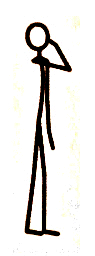
\includegraphics[width=0.7\linewidth]{water.jpg}
\column{.8\textwidth} % Right column and width
Water is an excellent \structure{conductor} for electrical energy. An optimal learning performance requires our \structure{hydration levels} to be \structure{balanced}. The water balances allows the \structure{efficient storage and retrieval of information} in the brain and in the body and activates \structure{optimal electrical and chemical processes} between the brain and the nervous system.
\end{columns}
\end{frame}
%------------------------------------------------
%----------------
%------------------------------------------------
\begin{frame}
\frametitle{Brain Buttons}


\begin{columns}[c] % The "c" option specifies centered vertical alignment while the "t" option is used for top vertical alignment

\column{.2\textwidth} % Left column and width
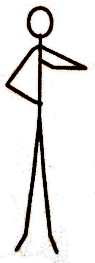
\includegraphics[width=0.7\linewidth]{buttons.jpg}
\column{.8\textwidth} % Right column and width
Hold one \structure{hand over the belly button} or massage a big area, \pause the other hand massages the \structure{points underneath the collarbone}, immediately left and right of the sternum on the first rib. \\
These are the end points of the kidney meridian (energy pathway in our body).
\note<1->{The hand on the \alert{belly button} brings the attention to the \structure{centre of gravity}. Here are the \structure{core muscles}, which are very important for the \structure{physical equilibrium}. The vestibular system gets activated, which \structure{readies the brain for incoming sensory input}.\\
If somebody is staring in the space in front of them (\structure{ocular blockage}), the \structure{vestibular activation} helps to get the \structure{eyes back to moving}.

}
\note<2->{It is assumed that \structure{increases the blood} flow through the main arteries into the brain by stimulating the arteries.The main arteries branch out from the hearth and bring \structure{fresh oxygen to the brain}. The buttons lie close to point where the main arteries fork. It is probably the \structure{baroreceptors} (pressure receptors) which are activated while rubbing these \alert{points}. \\ Baroreceptors react to a change in blood pressure and regulate a normal flow of blood to the brain.}
\end{columns}
\end{frame}
%------------------------------------------------
\begin{frame}
\frametitle{Brain Buttons: Effects on the body}
\begin{columns}[c] % The "c" option specifies centered vertical alignment while the "t" option is used for top vertical alignment

\column{.2\textwidth} % Left column and width
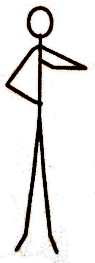
\includegraphics[width=0.7\linewidth]{buttons.jpg}
\column{.8\textwidth} % Right column and width
	\begin{itemize}
	\item[-] The hemispheres of the brain get centered and energetically charged.
	\item[-] The perception of the surroundings is sharpened.
	\item[-] Improves your awake state.
	\item[-] Hand--eye coordination improves.
	\item[-] Getting up in the morning gets easier, if done beforehand.
	\end{itemize}
\end{columns}
\end{frame}
%------------------------------------------------
\begin{frame}
\frametitle{Crossover Movement}


\begin{columns}[c] % The "c" option specifies centered vertical alignment while the "t" option is used for top vertical alignment

\column{.28\textwidth} % Left column and width
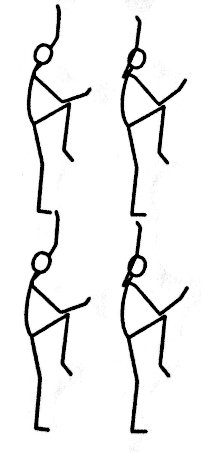
\includegraphics[width=1\linewidth]{crossover.jpg}
\column{.8\textwidth} % Right column and width
\textbf<1, 4>{\structure{Cross over 10 times}} (alternating: right elbow to the left knee and then left elbow to the right knee, 5 times each) while keeping your head steady and having the \structure{eyes in the upper left corner}. \pause

\textbf<2, 4>{\structure{Same side 10 times}} (right elbow to right knee alternated with other side, 5 times each) \structure{eyes in the lower right corner}. \pause

\textbf<3, 4>{\structure{Alternating:}} 1 time cross over, each direction once, eyes left up. 1 time same side, each side once, eyes down right. Repeat this 4 times, gives 16 movements. \pause
 
\textbf<4>{\structure{Possible progression:}} Again 16 times cross over with eyes closed.

\note<1->{The cross over movement should be should be \alert{executed very slowly}. A slow execution uses \structure{fine motorics} and \structure{balance} more and this leads to an activation of the \structure{vestibular system} and the \structure{frontal lobe}. The more fine motorics involved, the more are the frontal lobes connects with basal ganglion of the limbic system and the cerebellum in the brainstem.}
\end{columns}
\end{frame}
%------------------------------------------------
%------------------------------------------------
\begin{frame}
\frametitle{Crossover: Effects on the body}

\begin{columns}[c] % The "c" option specifies centered vertical alignment while the "t" option is used for top vertical alignment
\column{.28\textwidth} % Left column and width
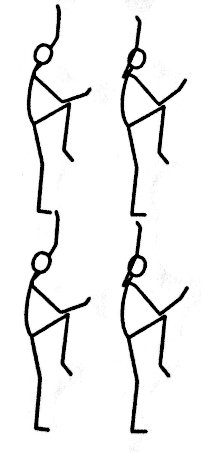
\includegraphics[width=1\linewidth]{crossover.jpg}
\column{.8\textwidth} % Right column and width
The crossover movement is a \structure{crossover walk in place}. It simultaneously activates big areas in \structure{both hemispheres} of the brain. This movement elegantly \structure{activates the whole brain} and even radiates into the frontal lobes. 

This movement is ideal to \structure{activate the body--mind system} before physical activities like sport or dancing.
\note{It is a \structure{conscious walking}, which stimulates the balanced neural activity across the \structure{corpus callosum}. If this happens on a regular base, more neural networks with stronger myelin layers form in the corpus callosum. This \structure{speeds up and integrates the communication between the hemispheres} and allows a \structure{higher--level thinking.}}
	\begin{itemize}
	\item[-] Optimizes attention, awareness and perception.
	\item[-] Language and expression become clear.
	\item[-] Eye and ear energy get balanced.
	\end{itemize}
	

\end{columns}
\end{frame}
%------------------------------------------------
%------------------------------------------------
\begin{frame}
\frametitle{Hook ups}


\begin{columns}[c] % The "c" option specifies centered vertical alignment while the "t" option is used for top vertical alignment

\column{.2\textwidth} % Left column and width
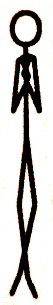
\includegraphics[width=0.4\linewidth]{Hookup.jpg}
\column{.8\textwidth} % Right column and width
Stand with \structure{legs crossed}, left over right, \structure{cross the arms} over in front of your body, interdigitate (interlock) your hands and bring them \structure{in front of your sternum}. Push the tongue flat against the roof of your mouth. \pause
\note<1->{The left ankle is put over the right ankle. The hands get crossed over, interlocked and turned around.

 To do so, reach out with your hands, put the \structure{back of the hands together}, thumbs are looking down. Keeping the orientation of the hands, put one over the other, palm to palm and \structure{interlock the hands} (interdigitate). Then \structure{turn} the interlocked \structure{hands down, towards the body}. They will eventually be \structure{in front of the sternum}, with the elbows facing down.
 
 The \alert{tongue against the roof of your mouth} connects the \structure{two main meridians} (the governor and the conception vessel) and it focusses the attention to the \structure{midbrain}, which lies above the roof of your mouth. It causes an \structure{increased tongue pressure} to decrease (caused by an unbalanced posture) and connects the emotions in the limbic system to the reason in the neocortex.
 
 Similar to the crossover movement, this \structure{integrates the hemispheres} and activates the \structure{sensor and motor areas} of the cortex in both hemispheres.}
\begin{itemize}
	\item[-] The meridians get connected and activated.
	\item[-] The emotions in the limbic system get connected to reason in the neocortex area.
	\item[-] Stimulates learning.
	\item[-] Stimulates effective action.
	\item[-] Centring, ex. during (or better before) an argument, bad feelings, ADHS, $\ldots$
	\end{itemize}
\note<2->{}
\end{columns}
\vspace{1cm}
Back to \href{run:./Exercises.pdf}{\underline{exercises}}.
\end{frame}
%------------------------------------------------

